\chapter{Parameterised Arrangements and Their Boundaries}

\section{A Family Is a Map From Parameters to Structure}

Chapter 11 introduced a family of nine-circle arrangements with two free parameters, the azimuth offset $\alpha$ and the elevation $\beta$ of the four flexible circles. A script that builds one member computes a single instance. A family is the map from the parameters to what is built, and the map has two kinds of output. The \emph{geometry}, the positions of the circles and vertices, varies continuously with $(\alpha,\beta)$. The \emph{combinatorial type}, the numbers of vertices, edges, and faces and the multiplicity of each vertex, takes finitely many values and changes only at certain parameter values. The parameter plane is therefore divided into regions on which the type is constant, which are the \emph{strata} of the family, separated by boundaries on which the type changes. Everything a reader needs to know about the family in order to choose a member is contained in the list of strata, where the boundaries lie, and what happens on them.

This chapter maps the family numerically, examines how a boundary behaves when it is approached, shows that the boundary that a computation reports depends on a tolerance and not only on the geometry, and builds a generator that produces named members from stored specifications and can be run twice without duplicating anything. The scripts are \texttt{param\_sweep.py} and \texttt{fig14\_boundary.py}, and the numbers come from runs in Blender 5.2.2's Python environment.

\section{Mapping the Parameter Space}

The family was sampled on a grid of one degree in both parameters, with $\alpha$ from $0^\circ$ to $90^\circ$ in $91$ values and $\beta$ from $1^\circ$ to $89^\circ$ in $89$ values, which is $8099$ members. For each member the vertices were found from the cross products of the normals and the numbers of vertices, edges, and faces and the histogram of multiplicities were recorded. The grid contained exactly two combinatorial types.

\begin{center}
\begin{tabular}{lrrrll}
\toprule
Type & $V$ & $E$ & $F$ & Multiplicities $\{m:\text{count}\}$ & Members on the grid\\
\midrule
Lattice & 26 & 72 & 48 & $\{2:12,\;3:8,\;4:6\}$ & 267\\
Generic & 54 & 116 & 64 & $\{2:48,\;3:4,\;4:2\}$ & 7832\\
\bottomrule
\end{tabular}
\end{center}

The lattice type occurs exactly at $\alpha=0^\circ$, $45^\circ$, and $90^\circ$ for every sampled $\beta$, which is $3\times89=267$ members. The generic type occurs at the other $88$ values of $\alpha$ for every $\beta$. No sampled member had two coincident circles and no member had a third type. The statement is about the grid. A thin set of exceptional parameter values that the grid steps over, for instance a value of $\beta$ between whole degrees at which some extra coincidence occurs, would not be seen, and the earlier mechanism analysis of Chapter 11 identifies two ways of coincidence and does not exclude others. The grid is evidence of a particular kind: it shows that exceptional values, if any, are not whole degrees, and it shows how the two types are arranged on the plane.

The picture of the strata is simple. The parameter plane has one generic stratum containing every sampled member off the lattice lines, and a set of lines $\alpha\in\{0,\pi/4,\pi/2\}$ carrying the lattice type. The lattice type is a higher-symmetry stratum of lower dimension. The count drops from $54$ to $26$ vertices when one moves onto a line, and the loss of $28$ vertices is accompanied by a gain in multiplicity: the generic arrangement has $2$ vertices of multiplicity four and the lattice arrangement has $6$.

\section{Approaching a Boundary}

The distinction between the strata can be made quantitative. Let $\delta$ be the distance of $\alpha$ from the nearest lattice value. As $\delta$ decreases the generic arrangement approaches the lattice one, and pairs of vertices that are distinct for $\delta>0$ approach each other and coincide at $\delta=0$. The smallest separation between two distinct vertices was measured at several values of $\delta$.

\begin{center}
\begin{tabular}{rrrr}
\toprule
$\delta$ (degrees) & Separation, $\beta=20^\circ$ & $\beta=35^\circ$ & $\beta=50^\circ$\\
\midrule
10 & $9.45\times10^{-2}$ & $1.39\times10^{-1}$ & $1.45\times10^{-1}$\\
1 & $1.05\times10^{-2}$ & $1.49\times10^{-2}$ & $1.46\times10^{-2}$\\
0.1 & $1.07\times10^{-3}$ & $1.51\times10^{-3}$ & $1.46\times10^{-3}$\\
0.01 & $1.07\times10^{-4}$ & $1.51\times10^{-4}$ & $1.46\times10^{-4}$\\
\bottomrule
\end{tabular}
\end{center}

The separation is proportional to $\delta$, and the constant of proportionality, with $\delta$ in radians, settles to $0.612$, $0.863$, and $0.839$ for $\beta=20^\circ$, $35^\circ$, and $50^\circ$. The left panel of Figure 14.1 shows the proportionality on logarithmic axes from $\delta=10^{-6}$ to $10^{-1}$. The geometry is continuous across the boundary, since a member close to the lattice line looks like a lattice member, and the combinatorial type is not: at $\delta=10^{-6}$ the members are visually indistinguishable from the lattice arrangement and have $54$ vertices where it has $26$.

\begin{figure}[ht]
\centering
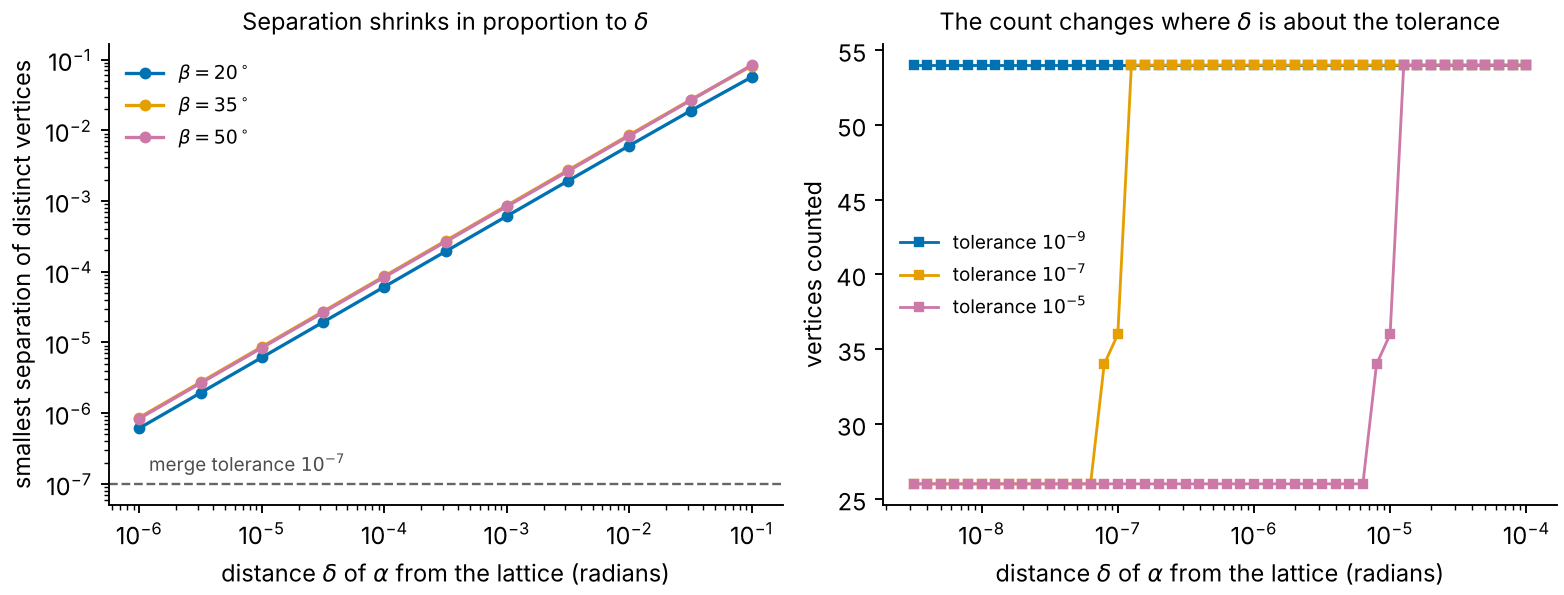
\includegraphics[width=\textwidth]{figs/fig14_boundary.png}
\caption{Left, the smallest separation of two distinct vertices against the distance $\delta$ of $\alpha$ from the lattice, for three values of $\beta$; the dashed line is a merge tolerance of $10^{-7}$. Right, the number of vertices counted at $\beta=35^\circ$ with three merge tolerances. The count drops from $54$ to $26$ where $\delta$ becomes comparable to the tolerance.}
\end{figure}

\section{A Boundary Depends on a Tolerance}

A count made by a program merges points closer than a tolerance, and so the count reports the type of the arrangement only when the tolerance is smaller than the separations that must be resolved and larger than the numerical noise. Near a boundary there is no such tolerance: the separation tends to zero, and any fixed tolerance eventually exceeds it. The right panel of Figure 14.1 shows the consequence. With a tolerance of $10^{-7}$ the count at $\beta=35^\circ$ was $54$ for $\delta\ge1.2\times10^{-7}$, $36$ and $34$ at $\delta=10^{-7}$ and $8\times10^{-8}$, and $26$ below. With a tolerance of $10^{-5}$ the same drop occurs at $\delta\approx10^{-5}$, and with $10^{-9}$ the count stayed at $54$ over the whole range plotted, which ends at $3\times10^{-9}$. The drop completes at about $1.2$ times the tolerance, in agreement with the measured $\delta$-to-separation ratio of $0.86$, and the two intermediate counts show that the vertex pairs merge at slightly different values of $\delta$, since the ratio varies from pair to pair.

The practical consequence concerns what an angle stored in the machine means. A value of $\alpha$ entered as $45^\circ$ in a field that stores single precision is not $\pi/4$ exactly: the stored value is $2.2\times10^{-8}$ radian above it, $90^\circ$ is $4.4\times10^{-8}$ above, and $135^\circ$ is $6\times10^{-9}$ above. For these three the vertex count was $54$ at a merge tolerance of $10^{-9}$ and $26$ at $10^{-7}$ and $10^{-6}$, so whether an arrangement entered on the lattice \emph{is} on the lattice depends on the tolerance of the program that counts it. For $22.5^\circ$ and $5^\circ$ the count was $54$ at all three tolerances. A report that says the arrangement at $\alpha=45^\circ$ has $26$ vertices is a report that the member, as stored, lies within the tolerance of the lattice line, and a careful report states the tolerance. This is the same lesson as the end of Chapter 13, applied to a parameter instead of a normal: the count is a function of the tolerance as well as of the arrangement, and a strata map should list the tolerances for which it is valid.

\section{Members From Specifications}

A generator that produces members of the family must record what it produced and must be safe to run twice. The function in \texttt{param\_sweep.py} builds a member into a collection named from its parameters, for example \texttt{Arrangement a22.5 b30}, stores the specification (parameters, sample count, radius) as a JSON string on the collection, stores the counts computed from the family formula beside it, stores each circle's unit normal on its object, and returns without doing anything if a collection of that name already exists. It was run on five specifications, $(\alpha,\beta)=(0,35)$, $(22.5,30)$, $(10,35)$, $(45,35)$, and $(5,35)$ in degrees, twice in succession.

\begin{center}
\begin{tabular}{lrrrrrr}
\toprule
Collection & $V$ & $E$ & $F$ & Rebuilt $V$ & $E$ & $F$\\
\midrule
\texttt{Arrangement a0 b35} & 26 & 72 & 48 & 26 & 72 & 48\\
\texttt{Arrangement a10 b35} & 54 & 116 & 64 & 54 & 116 & 64\\
\texttt{Arrangement a22.5 b30} & 54 & 116 & 64 & 54 & 116 & 64\\
\texttt{Arrangement a45 b35} & 26 & 72 & 48 & 26 & 72 & 48\\
\texttt{Arrangement a5 b35} & 54 & 116 & 64 & 54 & 116 & 64\\
\bottomrule
\end{tabular}
\end{center}

The first run created five collections, $45$ objects, and $45$ curve datablocks. The second created nothing and left the counts unchanged, which is the idempotence demonstrated for a different script in Chapter 6. The columns on the right were recomputed from the unit normals stored on the objects, without reference to the parameters, and agreed with the counts recorded at construction. The stored normals differed from the family formula's by up to $3\times10^{-8}$, because Blender stores the vectors in single precision, and this is within the window of tolerances found in Chapter 13. The member can therefore be reconstructed from the record in two independent ways, from its specification by the formula and from its stored normals by direct count, and the two agree. What the record does not contain is the tolerance used in counting, and it should, for the reason of the previous section.

\section{What a Sweep Report Should Contain}

A report on a sweep of a parameterised family should state the grid, the list of types found with their counts and the number of grid members of each, the locations of the boundaries between types and a description of how each is approached, and the tolerance under which the counts were made along with the window of tolerances in which they are stable. For this family the report reads: on a one-degree grid there are two types, the lattice type on three lines and the generic type elsewhere; the separation of the vertex pairs that merge is proportional to the distance from the lattice with a constant between $0.6$ and $0.9$; and counts from single-precision data are correct between a tolerance of a few times $10^{-7}$ and about $0.25$, except within a few times the tolerance of the boundary itself, where the count is not an invariant of the geometry.

\begin{exercise}[14.1: A finer grid]
Refine the grid to $0.25^\circ$ in $\beta$ and $2.5^\circ$ in $\alpha$ near $\beta=45^\circ$ and $\beta=60^\circ$, and report whether any third combinatorial type appears. State what a result of ``none'' does and does not establish.
\end{exercise}

\begin{exercise}[14.2: Predict the flip]
For $\beta=50^\circ$ predict, from the measured constant, the value of $\delta$ at which the count at tolerance $10^{-6}$ begins to fall from $54$, and then measure it.
\end{exercise}

\begin{exercise}[14.3: Store the tolerance]
Add the counting tolerance to the stored record of \texttt{param\_sweep.py} and make the reconstruction step report the interval of tolerances over which the rebuilt counts equal the recorded ones.
\end{exercise}

\begin{exercise}[14.4: A third parameter]
Let the polar circles' azimuths be $k\pi/4+\gamma$ for a parameter $\gamma$. Predict which values of $\gamma$ will change the combinatorial type, using the two mechanisms of Chapter 11, and test the prediction on a grid.
\end{exercise}
